% Options for packages loaded elsewhere
\PassOptionsToPackage{unicode}{hyperref}
\PassOptionsToPackage{hyphens}{url}
\PassOptionsToPackage{dvipsnames,svgnames,x11names}{xcolor}
\documentclass[
  10pt,
  fontset=fandol]{ctexart}
\usepackage{xcolor}
\usepackage[margin=16mm]{geometry}
\usepackage{amsmath,amssymb}
\setcounter{secnumdepth}{-\maxdimen} % remove section numbering
\usepackage{iftex}
\ifPDFTeX
  \usepackage[T1]{fontenc}
  \usepackage[utf8]{inputenc}
  \usepackage{textcomp} % provide euro and other symbols
\else % if luatex or xetex
  \usepackage{unicode-math} % this also loads fontspec
  \defaultfontfeatures{Scale=MatchLowercase}
  \defaultfontfeatures[\rmfamily]{Ligatures=TeX,Scale=1}
\fi
\usepackage{lmodern}
\ifPDFTeX\else
  % xetex/luatex font selection
\fi
% Use upquote if available, for straight quotes in verbatim environments
\IfFileExists{upquote.sty}{\usepackage{upquote}}{}
\IfFileExists{microtype.sty}{% use microtype if available
  \usepackage[]{microtype}
  \UseMicrotypeSet[protrusion]{basicmath} % disable protrusion for tt fonts
}{}
\makeatletter
\@ifundefined{KOMAClassName}{% if non-KOMA class
  \IfFileExists{parskip.sty}{%
    \usepackage{parskip}
  }{% else
    \setlength{\parindent}{0pt}
    \setlength{\parskip}{6pt plus 2pt minus 1pt}}
}{% if KOMA class
  \KOMAoptions{parskip=half}}
\makeatother
\usepackage{longtable,booktabs,array}
\newcounter{none} % for unnumbered tables
\usepackage{calc} % for calculating minipage widths
% Correct order of tables after \paragraph or \subparagraph
\usepackage{etoolbox}
\makeatletter
\patchcmd\longtable{\par}{\if@noskipsec\mbox{}\fi\par}{}{}
\makeatother
% Allow footnotes in longtable head/foot
\IfFileExists{footnotehyper.sty}{\usepackage{footnotehyper}}{\usepackage{footnote}}
\makesavenoteenv{longtable}
\usepackage{graphicx}
\makeatletter
\newsavebox\pandoc@box
\newcommand*\pandocbounded[1]{% scales image to fit in text height/width
  \sbox\pandoc@box{#1}%
  \Gscale@div\@tempa{\textheight}{\dimexpr\ht\pandoc@box+\dp\pandoc@box\relax}%
  \Gscale@div\@tempb{\linewidth}{\wd\pandoc@box}%
  \ifdim\@tempb\p@<\@tempa\p@\let\@tempa\@tempb\fi% select the smaller of both
  \ifdim\@tempa\p@<\p@\scalebox{\@tempa}{\usebox\pandoc@box}%
  \else\usebox{\pandoc@box}%
  \fi%
}
% Set default figure placement to htbp
\def\fps@figure{htbp}
\makeatother
\setlength{\emergencystretch}{3em} % prevent overfull lines
\providecommand{\tightlist}{%
  \setlength{\itemsep}{0pt}\setlength{\parskip}{0pt}}
\usepackage{amsmath,amssymb,mathtools,needspace}
\xeCJKDeclareCharClass{CJK}{"2032,"0400->"04FF,"2160->"216B,"2460->"2473,"25A0,"25C7,"25CB,"25CF}
\IfFontExistsTF{Arial Unicode MS}{\xeCJKsetup{AutoFallBack=true}\setCJKfallbackfamilyfont{\CJKrmdefault}{Arial Unicode MS}}{}
\setcounter{secnumdepth}{0}
\setlength{\emergencystretch}{2em}
\allowdisplaybreaks
\usepackage{bookmark}
\IfFileExists{xurl.sty}{\usepackage{xurl}}{} % add URL line breaks if available
\urlstyle{same}
\hypersetup{
  pdftitle={曲线拟合的最小二乘法},
  colorlinks=true,
  linkcolor={Maroon},
  filecolor={Maroon},
  citecolor={Blue},
  urlcolor={Blue},
  pdfcreator={LaTeX via pandoc}}

\title{曲线拟合的最小二乘法}
\author{}
\date{}

\begin{document}
\maketitle

\subsection{3.6 曲线拟合的最小二乘法}\label{ux66f2ux7ebfux62dfux5408ux7684ux6700ux5c0fux4e8cux4e58ux6cd5}

\subsubsection{3.6.1 一般的最小二乘逼近}\label{ux4e00ux822cux7684ux6700ux5c0fux4e8cux4e58ux903cux8fd1}

在科学实验的统计方法研究中，往往要从一组实验数据 \((x_i,y_i)\)（\(i=0,1,\cdots,m\)）中寻找自变量 \(x\) 与因变量 \(y\) 之间的函数关系 \(y=F(x)\)。由于观测数据往往不准确，因此不要求 \(y=F(x)\) 经过所有点 \((x_i,y_i)\)，而只要求在给定点 \(x_i\) 上误差 \(\delta_i=F(x_i)-y_i\)（\(i=0,1,\cdots,m\)）按某种标准最小。若记 \(\boldsymbol\delta=(\delta_0,\delta_1,\cdots,\delta_m)^{\mathrm T}\)，就是要求向量 \(\boldsymbol\delta\) 的范数 \(\|\boldsymbol\delta\|\) 最小。如果用最大范数，计算上困难较大，通常就采用 Euclid 范数 \(\|\boldsymbol\delta\|_2\) 作为误差度量的标准。关于最小二乘法的一般提法是：对于给定的一组数据 \((x_i,y_i)\)（\(i=0,1,\cdots,m\)），要求在函数空间 \(\Phi=\operatorname{span}\{\varphi_0,\varphi_1,\cdots,\varphi_n\}\) 中找一个函数 \(y=S^*(x)\)，使误差平方和

\begin{quote}
校注（agent 补充）：本页最大误差式原书写 \(S_3(x)\)，而同例的最佳平方逼近多项式记作 \(S_3^*(x)\)；转录保留原来的无星号记法。
\end{quote}

\href{../../source-images/pdf-079.jpeg}{查看原页}

\[
\|\boldsymbol\delta\|_2^2=\sum_{i=0}^m\delta_i^2=\sum_{i=0}^m[S^*(x_i)-y_i]^2=\min_{S(x)\in\varphi}\sum_{i=1}^m[S(x_i)-y_i]^2,\tag{3.6.1}
\]

这里

\[
S(x)=a_0\varphi_0(x)+a_1\varphi_1(x)+\cdots+a_n\varphi_n(x)\quad(n<m).\tag{3.6.2}
\]

这就是一般的最小二乘逼近，用几何语言说，就称为曲线拟合的最小二乘法。

用最小二乘法求拟合曲线时，首先要确定 \(S(x)\) 的形式。这不是单纯数学问题，还与所研究问题的运动规律及所得观测数据 \((x_i,y_i)\) 有关；通常要从问题的运动规律及给定数据描图来确定 \(S(x_i)\) 的形式，并通过实际计算选出较好的结果------这点将从下面的例题得到说明。\(S(x)\) 的一般表达式为式 (3.6.2) 所示的线性形式。若 \(\varphi_k(x)\) 是 \(k\) 次多项式，\(S(x)\) 就是 \(n\) 次多项式。为了使问题的提法更有一般性，通常把最小二乘法中 \(\|\boldsymbol\delta\|_2^2\) 都考虑为加权平方和

\[
\|\boldsymbol\delta\|_2^2=\sum_{i=0}^m\omega(x_i)[S(x_i)-f(x_i)]^2.\tag{3.6.3}
\]

这里 \(\omega(x)\geqslant0\) 是 \([a,b]\) 上的权函数，它表示不同点 \((x_i,f(x_i))\) 处的数据比重不同，例如，\(\omega(x_i)\) 可表示在点 \((x_i,f(x_i))\) 处重复观测的次数。用最小二乘法求拟合曲线的问题，就是在形如式 (3.6.2) 的 \(S(x)\) 中求一函数 \(y=S^*(x)\)，使式 (3.6.3) 取得最小。它转化为求多元函数

\[
I(a_0,a_1,\cdots,a_n)=\sum_{i=0}^m\omega(x_i)\left[\sum_{j=0}^na_j\varphi_j(x_i)-f(x_i)\right]^2\tag{3.6.4}
\]

的极小点 \((a_0^*,a_1^*,\cdots,a_n^*)\) 问题。这与 3.3 节讨论的问题完全类似。由求多元函数极值的必要条件，有

\[
\frac{\partial I}{\partial a_k}=2\sum_{i=0}^m\omega(x_i)\left[\sum_{j=0}^na_j\varphi_j(x_i)-f(x_i)\right]\varphi_k(x_i)=0\quad(k=0,1,\cdots,n).
\]

若记

\[
(\varphi_j,\varphi_k)=\sum_{i=0}^m\omega(x_i)\varphi_j(x_i)\varphi_k(x_i),\tag{3.6.5}
\]

则

\[
(f,\varphi_k)=\sum_{i=0}^m\omega(x_i)f(x_i)\varphi_k(x_i)\equiv d_k\quad(k=0,1,\cdots,n),
\]

可改写为

\[
\sum_{j=0}^n(\varphi_k,\varphi_j)a_j=d_k\quad(k=0,1,\cdots,n).\tag{3.6.6}
\]

此方程称为法方程。它也可写成矩阵形式

\[
G\boldsymbol a=\boldsymbol d,
\]

其中

\[
\boldsymbol a=(a_0,a_1,\cdots,a_n)^{\mathrm T},\quad\boldsymbol d=(d_0,d_1,\cdots,d_n)^{\mathrm T},
\]

\[
G=\begin{pmatrix}
(\varphi_0,\varphi_0)&(\varphi_0,\varphi_1)&\cdots&(\varphi_0,\varphi_n)\\
(\varphi_1,\varphi_0)&(\varphi_1,\varphi_1)&\cdots&(\varphi_1,\varphi_n)\\
\vdots&\vdots&&\vdots\\
(\varphi_n,\varphi_0)&(\varphi_n,\varphi_1)&\cdots&(\varphi_n,\varphi_n)
\end{pmatrix},\tag{3.6.7}
\]

\begin{quote}
校注（agent 补充）：式 (3.6.1) 右端原书求和下限明确为 \(i=1\)，其左侧两个求和及本节数据下标均从 \(i=0\) 开始；原式已保留，右端下限疑应为 \(i=0\)。最小值的下标原书印为 \(S(x)\in\varphi\)（小写），而前页函数空间记为 \(\Phi\)，此处亦保留原印字形。见 \href{../assets/ch03b/p079-minimum-formula.png}{原式放大裁切}。
\end{quote}

\href{../../source-images/pdf-080.jpeg}{查看原页}

由于 \(\varphi_0,\varphi_1,\cdots,\varphi_n\) 线性无关，故 \(|G|\ne0\)，方程组 (3.6.6) 存在唯一的解

\[
a_k=a_k^*\quad(k=0,1,\cdots,n),
\]

从而得到函数 \(f(x)\) 的最小二乘解为

\[
S^*(x)=a_0^*\varphi_0(x)+a_1^*\varphi_1(x)+\cdots+a_n^*\varphi_n(x).
\]

可以证明，这样得到的 \(S^*(x)\) 对于任何形如式 (3.6.2) 的 \(S(x)\)，都有

\[
\sum_{i=0}^m\omega(x_i)[S^*(x_i)-f(x_i)]^2\leqslant\sum_{i=0}^m\omega(x_i)^*[S(x_i)-f(x_i)]^2,
\]

故 \(S^*(x)\) 确是所求最小二乘解。它的证明与式 (3.3.14) 相似，读者可自己完成。

\textbf{例 3.5} 已知一组实验数据如表 3.3 所示，求它的拟合曲线。

\textbf{表 3.3}

{\def\LTcaptype{none} % do not increment counter
\begin{longtable}[]{@{}lrrrrr@{}}
\toprule\noalign{}
\(x_i\) & 1 & 2 & 3 & 4 & 5 \\
\midrule\noalign{}
\endhead
\bottomrule\noalign{}
\endlastfoot
\(f_i\) & 4 & 4.5 & 6 & 8 & 8.5 \\
\(\omega_i\) & 2 & 1 & 3 & 1 & 1 \\
\end{longtable}
}

\textbf{解} 在坐标纸上标出所给数据，如图 3.6 所示。从图 3.6 可看到，各点分布在一条直线附近，故可选择线性函数作拟合曲线。令 \(S_1(x)=a_0+a_1x\)，这里 \(m=4,n=1,\varphi_0(x)=1,\varphi_1(x)=x\)，故

\[
(\varphi_0,\varphi_0)=\sum_{i=0}^4\omega_i=8,\quad(\varphi_0,\varphi_1)=(\varphi_1,\varphi_0)=\sum_{i=0}^4\omega_ix_i=22,
\]

\[
(\varphi_1,\varphi_1)=\sum_{i=0}^4\omega_ix_i^2=74,\quad(\varphi_0,f)=\sum_{i=0}^4\omega_if_i=47,
\]

\[
(\varphi_1,f)=\sum_{i=0}^4\omega_ix_if_i=145.5.
\]

由式 (3.6.6) 得方程组

\[
\begin{cases}
8a_0+22a_1=47,\\
22a_0+74a_1=145.5,
\end{cases}
\]

解得

\[
a_0=2.77,\quad a_1=1.13.
\]

于是所求拟合曲线为

\[
S_1^*(x)=2.77+1.13x.
\]

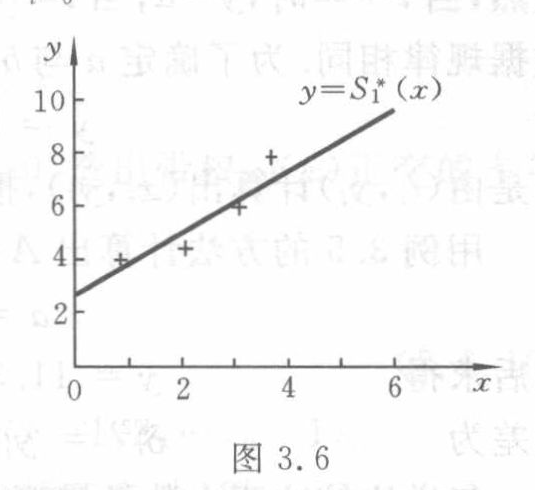
\includegraphics[width=0.85\linewidth,height=\textheight,keepaspectratio,alt={图 3.6（原图裁切）}]{../assets/ch03b/figure-3-6.png}

\textbf{图 3.6}（原图裁切）。图中以十字标记数据点，并画出拟合直线 \(y=S_1^*(x)\)。图中文字与符号：\(x,y,0\)；横轴标值 \(2,4,6\)，纵轴标值 \(2,4,6,8,10\)；曲线标签 \(y=S_1^*(x)\)。

\textbf{例 3.6} 在某化学反应过程中，根据实验所得生成物的质量分数与时间的关系如表 3.4 所示，求质量分数 \(y\) 与时间 \(t\) 的拟合曲线 \(y=F(t)\)。

\textbf{表 3.4}

{\def\LTcaptype{none} % do not increment counter
\begin{longtable}[]{@{}
  >{\raggedright\arraybackslash}p{(\linewidth - 32\tabcolsep) * \real{0.0448}}
  >{\raggedleft\arraybackslash}p{(\linewidth - 32\tabcolsep) * \real{0.0597}}
  >{\raggedleft\arraybackslash}p{(\linewidth - 32\tabcolsep) * \real{0.0597}}
  >{\raggedleft\arraybackslash}p{(\linewidth - 32\tabcolsep) * \real{0.0597}}
  >{\raggedleft\arraybackslash}p{(\linewidth - 32\tabcolsep) * \real{0.0597}}
  >{\raggedleft\arraybackslash}p{(\linewidth - 32\tabcolsep) * \real{0.0597}}
  >{\raggedleft\arraybackslash}p{(\linewidth - 32\tabcolsep) * \real{0.0597}}
  >{\raggedleft\arraybackslash}p{(\linewidth - 32\tabcolsep) * \real{0.0597}}
  >{\raggedleft\arraybackslash}p{(\linewidth - 32\tabcolsep) * \real{0.0597}}
  >{\raggedleft\arraybackslash}p{(\linewidth - 32\tabcolsep) * \real{0.0597}}
  >{\raggedleft\arraybackslash}p{(\linewidth - 32\tabcolsep) * \real{0.0597}}
  >{\raggedleft\arraybackslash}p{(\linewidth - 32\tabcolsep) * \real{0.0597}}
  >{\raggedleft\arraybackslash}p{(\linewidth - 32\tabcolsep) * \real{0.0597}}
  >{\raggedleft\arraybackslash}p{(\linewidth - 32\tabcolsep) * \real{0.0597}}
  >{\raggedleft\arraybackslash}p{(\linewidth - 32\tabcolsep) * \real{0.0597}}
  >{\raggedleft\arraybackslash}p{(\linewidth - 32\tabcolsep) * \real{0.0597}}
  >{\raggedleft\arraybackslash}p{(\linewidth - 32\tabcolsep) * \real{0.0597}}@{}}
\toprule\noalign{}
\begin{minipage}[b]{\linewidth}\raggedright
\(t/\mathrm{min}\)
\end{minipage} & \begin{minipage}[b]{\linewidth}\raggedleft
1
\end{minipage} & \begin{minipage}[b]{\linewidth}\raggedleft
2
\end{minipage} & \begin{minipage}[b]{\linewidth}\raggedleft
3
\end{minipage} & \begin{minipage}[b]{\linewidth}\raggedleft
4
\end{minipage} & \begin{minipage}[b]{\linewidth}\raggedleft
5
\end{minipage} & \begin{minipage}[b]{\linewidth}\raggedleft
6
\end{minipage} & \begin{minipage}[b]{\linewidth}\raggedleft
7
\end{minipage} & \begin{minipage}[b]{\linewidth}\raggedleft
8
\end{minipage} & \begin{minipage}[b]{\linewidth}\raggedleft
9
\end{minipage} & \begin{minipage}[b]{\linewidth}\raggedleft
10
\end{minipage} & \begin{minipage}[b]{\linewidth}\raggedleft
11
\end{minipage} & \begin{minipage}[b]{\linewidth}\raggedleft
12
\end{minipage} & \begin{minipage}[b]{\linewidth}\raggedleft
13
\end{minipage} & \begin{minipage}[b]{\linewidth}\raggedleft
14
\end{minipage} & \begin{minipage}[b]{\linewidth}\raggedleft
15
\end{minipage} & \begin{minipage}[b]{\linewidth}\raggedleft
16
\end{minipage} \\
\midrule\noalign{}
\endhead
\bottomrule\noalign{}
\endlastfoot
\(y/\times10^{-3}\) & 4.00 & 6.40 & 8.00 & 8.80 & 9.22 & 9.50 & 9.70 & 9.86 & 10.00 & 10.20 & 10.32 & 10.42 & 10.50 & 10.55 & 10.58 & 10.60 \\
\end{longtable}
}

\textbf{解} 将所给数据标在坐标纸上，如图 3.7 所示。可以看到，质量分数开始时增加较快，后来逐渐减慢，到一定时间就基本稳定在一个水平上，即当 \(t\to\infty\) 时，\(y\) 趋于某

\begin{quote}
校注（agent 补充）：最小二乘不等式右端的 \(\omega(x_i)\) 后原书印有上标星号，原式已保留。该星号在权函数定义中没有定义，疑为多余印字；与式 (3.6.3) 的一致写法应为 \(\omega(x_i)[S(x_i)-f(x_i)]^2\)。见 \href{../assets/ch03b/p080-minimum-inequality.png}{原式放大裁切}。
\end{quote}

\href{../../source-images/pdf-081.jpeg}{查看原页}

个数，故 \(y=F(t)\) 有一水平渐近线。另外，\(t=0\) 时，反应未开始，质量分数为零。根据这些特点，可设想 \(y=F(t)\) 是双曲线型 \(1/y=a+b/t\)，即 \(y=t/(at+b)\)。它与给定数据的规律大致符合。

为了确定 \(a,b\)，令 \(\bar y=1/y,x=1/t\)，于是可用 \(x\) 的线性函数 \(S_1(x)=a+bx\) 拟合数据 \((x_i,\bar y_i)\)（\(i=1,2,\cdots,16\)），\(x_i,\bar y_i\) 由原始数据 \((t_i,y_i)\) 根据变换计算出来。与例 3.5 方法相同，解方程组

\[
\begin{cases}
16a+3.38073b=1.8372\times10^3,\\
3.38073a+1.58435b=0.52886\times10^3,
\end{cases}
\]

得

\[
a=80.6621,\quad b=161.6822.
\]

从而得到

\[
y=t/(80.6621t+161.6822)=F^{(1)}(t),
\]

其误差为

\[
\delta_i^{(1)}=y_i-F^{(1)}(t_i)\quad(i=1,2,\cdots,16).
\]

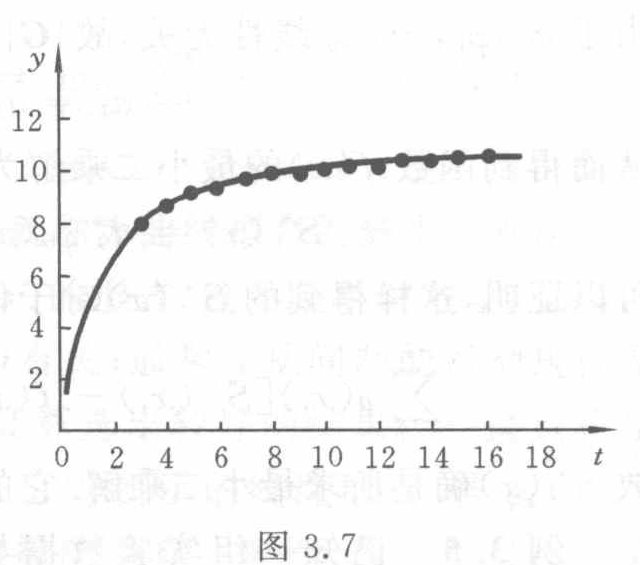
\includegraphics[width=0.85\linewidth,height=\textheight,keepaspectratio,alt={图 3.7（原图裁切）}]{../assets/ch03b/figure-3-7.png}

\textbf{图 3.7}（原图裁切）。实验数据点及逐渐趋于水平的拟合曲线。图中文字与符号：纵轴 \(y\)，横轴 \(t\)，原点 \(0\)；横轴标值 \(2,\allowbreak 4,\allowbreak 6,\allowbreak 8,\allowbreak 10,\allowbreak 12,\allowbreak 14,\allowbreak 16,\allowbreak 18\)，纵轴标值 \(2,\allowbreak 4,\allowbreak 6,\allowbreak 8,\allowbreak 10,\allowbreak 12\)。

由图 3.7，符合给定数据的函数还可选为指数形式。此时可令拟合曲线形如

\[
y=a\mathrm e^{b/t}.
\]

显然，当 \(t\to\infty\) 时，\(y\to a\)；当 \(t\to0\) 时，若 \(b<0\)，则 \(y\to0\)，且 \(t\) 增加时 \(y\) 增加。这些与给出数据规律相同。为了确定 \(a\) 与 \(b\)，对上式两端取对数，得 \(\ln y=\ln a+b/t\)。令

\[
\hat y=\ln y,\quad A=\ln a,\quad x=1/t,
\]

于是由 \((t_i,y_i)\) 计算出 \((x_i,\hat y_i)\)，拟合数据 \((x_i,y_i)\) 的曲线仍为 \(S_1(x)=A+bx\)。

用例 3.5 的方法计算出 \(A=-4.48072,b=-1.0567\)，从而

\[
a=\mathrm e^A=11.3253\times10^{-3},
\]

最后求得

\[
y=11.3253\times10^{-3}\mathrm e^{-1.0567t}=F^{(2)}(t),
\]

误差为

\[
\delta_i^{(2)}=y_i-F^{(2)}(t_i)\quad(i=1,2,\cdots,16).
\]

怎样比较这两个数学模型的好坏呢？只要分别计算各点误差，从中挑选误差较小的模型即可。本例经过计算可得

\[
\|\boldsymbol\delta^{(1)}\|_\infty=\max_i|\delta_i^{(1)}|=0.568\times10^{-3},
\]

\[
\|\boldsymbol\delta^{(2)}\|_\infty=\max_i|\delta_i^{(2)}|=0.277\times10^{-3},
\]

而均方误差为

\[
\|\boldsymbol\delta^{(1)}\|_2=\sqrt{\sum_{i=1}^m(\delta_i^{(1)})^2}=1.19\times10^{-3},
\]

\[
\|\boldsymbol\delta^{(2)}\|_2=\sqrt{\sum_{i=1}^m(\delta_i^{(2)})^2}=0.34\times10^{-3},
\]

\begin{quote}
校注（agent 补充）：本页最终 \(F^{(2)}(t)\) 的原书指数明确印为 \(-1.0567t\)，已保留。由上文设定 \(y=a\mathrm e^{b/t}\) 及 \(b=-1.0567\)，相容表达式应为 \(\mathrm e^{-1.0567/t}\)；前者在 \(t\to\infty\) 时趋于零，与本页给出的模型性质和数据不相容，属疑似原书漏印除号。见 \href{../assets/ch03b/p081-exponential-fit.png}{原式放大裁切}。上文``拟合数据 \((x_i,y_i)\)''亦按原印保留，其语境对应的是变换后的 \((x_i,\hat y_i)\)。
\end{quote}

\href{../../source-images/pdf-082.jpeg}{查看原页}

由此可知，\(\|\boldsymbol\delta^{(2)}\|_2\) 及 \(\|\boldsymbol\delta^{(2)}\|_\infty\) 都比较小，所以用 \(y=F^{(2)}(t)\) 作拟合曲线比较好。

从本例看到，拟合曲线的数学模型并不是一开始就能选得好的，往往要通过分析确定若干模型后，再经过实际计算，才能选到较好的模型。本例的指数模型就比双曲线模型好。

现在很多计算机配有自动选择数学模型的程序，其方法与本例相同。程序中因变量与自变量变换的函数类型较多，通过计算比较误差找到拟合得较好的曲线，最后输出曲线图形及数学表达式。

\subsubsection{3.6.2 用正交函数作最小二乘拟合}\label{ux7528ux6b63ux4ea4ux51fdux6570ux4f5cux6700ux5c0fux4e8cux4e58ux62dfux5408}

用最小二乘法得到的法方程组 (3.6.6)，其系数矩阵 \(G\) 是病态的，但如果 \(\varphi_0(x),\varphi_1(x),\cdots,\varphi_n(x)\) 是关于点集 \(\{x_i\}\)（\(i=0,1,\cdots,m\)）带权 \(\omega(x_i)\)（\(i=0,1,\cdots,m\)）正交的函数族，即

\[
(\varphi_j,\varphi_k)=\sum_{i=0}^m\omega(x_i)\varphi_j(x_i)\varphi_k(x_i)=\begin{cases}0,&j\ne k,\\ A_k>0,&j=k,\end{cases}\tag{3.6.8}
\]

则方程组 (3.6.6) 的解为

\[
a_k^*=\frac{(f,\varphi_k)}{(\varphi_k,\varphi_k)}=\frac{\displaystyle\sum_{i=0}^m\omega(x_i)f(x_i)\varphi_k(x_i)}{\displaystyle\sum_{i=0}^m\omega(x_i)\varphi_k^2(x_i)}\quad(k=0,1,\cdots,n),\tag{3.6.9}
\]

且平方误差为

\[
\|\delta\|_2^2=\|f\|_2^2-\sum_{k=0}^n A_k(a_k^*)^2.
\]

现在根据给定节点 \(x_0,x_1,\cdots,x_m\) 及权函数 \(\omega(x)>0\)，造出带权 \(\omega(x)\) 正交的多项式 \(\{P_n(x)\}\)。注意 \(n\leqslant m\)，用递推公式表示 \(P_k(x)\)，即

\[
\begin{cases}
P_0(x)=1,\\
P_1(x)=(x-\alpha_1)P_0(x),\\
P_{k+1}(x)=(x-\alpha_{k+1})P_k(x)-\beta_kP_{k-1}(x)\quad(k=1,2,\cdots,n-1).
\end{cases}\tag{3.6.10}
\]

这里 \(P_k(x)\) 是首项系数为 \(1\) 的 \(k\) 次多项式。根据 \(P_k(x)\) 的正交性，得

\[
\left\{\begin{aligned}
a_{k+1}&=\frac{\displaystyle\sum_{i=0}^m\omega(x_i)x_iP_k^2(x_i)}{\displaystyle\sum_{i=0}^m\omega(x_i)P_k^2(x_i)}=\frac{(xP_k(x),P_k(x))}{(P_k(x),P_k(x))}=\frac{(xP_k,P_k)}{(P_k,P_k)},\\
\beta_k&=\frac{\displaystyle\sum_{i=0}^m\omega(x_i)P_k^2(x_i)}{\displaystyle\sum_{i=0}^m\omega(x_i)P_{k-1}^2(x_i)}=\frac{(P_k,P_k)}{(P_{k-1},P_{k-1})}
\end{aligned}\right.\quad(k=0,1,\cdots,n-1).\tag{3.6.11}
\]

\begin{quote}
校注（agent 补充）：式 (3.6.11) 第一行原书印为拉丁字母 \(a_{k+1}\)，式 (3.6.10) 则为希腊字母 \(\alpha_{k+1}\)，已分别保留。该式末的共同范围原书为 \(k=0,1,\cdots,n-1\)；若直接用于第二行 \(\beta_k\)，\(k=0\) 会涉及未定义的 \(P_{-1}\)。依式 (3.6.10)，实际递推使用的是 \(\beta_1,\ldots,\beta_{n-1}\)。见 \href{../assets/ch03b/p082-recursion-coefficients.png}{原式裁切}。
\end{quote}

\href{../../source-images/pdf-083.jpeg}{查看原页}

下面用归纳法证明这样给出的 \(\{P_k(x)\}\) 是正交的。由式 (3.6.10) 第二式及式 (3.6.11) 中 \(a_1\) 的表达式，有

\[
\begin{aligned}
(P_l,P_1)&=(P_0,xP_0)-\alpha_1(P_0,P_0)\\
&=(P_0,xP_0)-\frac{(xP_0,P_0)}{(P_0,P_0)}(P_0,P_0)=0.
\end{aligned}
\]

现假定 \((P_1,P_s)=0\)（\(l\ne s\)）对于 \(s=0,1,\cdots,l-1\) 及 \(l=0,1,\cdots,k\)（\(k<n\)）均成立，要证 \((P_{k+1},P_s)=0\) 对于 \(s=0,1,\cdots,k\) 均成立。由式 (3.6.10)，有

\[
\begin{aligned}
(P_{k+1},P_s)&=((x-\alpha_{k+1})P_k,P_s)-\beta_k(P_{k-1},P_s)\\
&=(xP_k,P_s)-\alpha_{k+1}(P_k,P_s)-\beta_k(P_{k-1},P_s),
\end{aligned}\tag{3.6.12}
\]

由归纳法假定，当 \(0\leqslant s\leqslant k-2\) 时

\[
(P_k,P_s)=0,\quad(P_{k-1},P_s)=0.
\]

另外，\(xP_s(x)\) 是首项系数为 \(1\) 的 \(s+1\) 次多项式，它可用 \(P_0,P_1,\cdots,P_{s+1}\) 的线性组合表示，而 \(s+1\leqslant k-1\)，故由归纳法假定又有

\[
(xP_k,P_s)\equiv(P_k,xP_s)=0,
\]

于是由式 (3.6.12)，当 \(s\leqslant k-2\) 时，\((P_{k+1},P_s)=0\)。

再看

\[
(P_{k+1},P_{k-1})=(xP_k,P_{k-1})-\alpha_{k+1}(P_k,P_{k-1})-\beta_k(P_{k-1},P_{k-1}),\tag{3.6.13}
\]

由假定有

\[
(P_k,P_{k-1})=0,
\]

\[
(xP_k,P_{k-1})=(P_k,xP_{k-1})=\left(P_k,P_k+\sum_{j=0}^{k-1}C_jP_j\right)=(P_k,P_k).
\]

利用式 (3.6.11) 的 \(\beta_k\) 表达式及以上结果，得

\[
(P_{k+1},P_{k-1})=(xP_k,P_{k-1})-\beta_k(P_{k-1},P_{k-1})=(P_k,P_k)-(P_k,P_k)=0.
\]

最后，由式 (3.6.11) 有

\[
\begin{aligned}
(P_{k+1},P_k)&=(xP_k,P_k)-\alpha_{k+1}(P_k,P_k)-\beta_k(P_k,P_{k-1})\\
&=(xP_k,P_k)-\frac{(xP_k,P_k)}{(P_k,P_k)}(P_k,P_k)=0.
\end{aligned}
\]

至此已证明了由式 (3.6.10) 及式 (3.6.11) 确定的多项式，\(\{P_k(x)\}\)（\(k=0,1,\cdots,n;n\leqslant m\)）组成一个关于点集 \(\{x_i\}\) 的正交系。

用正交多项式 \(\{P_k(x)\}\) 的线性组合作最小二乘曲线拟合，只要在根据式 (3.6.10) 及式 (3.6.11) 逐步求 \(P_k(x)\) 的同时，相应计算出系数

\[
a_k=\frac{(f,P_k)}{(P_k,P_k)}=\frac{\displaystyle\sum_{i=0}^m\omega(x_i)f(x_i)P_k(x_i)}{\displaystyle\sum_{i=0}^m\omega(x_i)P_k^2(x_i)}\quad(k=0,1,\cdots,n),
\]

并逐步把 \(\alpha_k^*P_k(x)\) 累加到 \(F(x)\) 中去，最后就可得到所求的拟合曲线

\[
y=F(x)=\alpha_0^*P_0(x)+\alpha_1^*P_1(x)+\cdots+\alpha_n^*P_n(x),
\]

\begin{quote}
校注（agent 补充）：本页第一式左端原扫描为 \((P_l,P_1)\)（第一下标为字母 \(l\)），依右端计算应对应 \((P_0,P_1)\)。下一段归纳假设原印为 \((P_1,P_s)=0\)，括号内条件却为 \(l\ne s\)，疑应为 \((P_l,P_s)=0\)。均忠实保留并见 \href{../assets/ch03b/p083-induction-start.png}{原文裁切}。页尾系数公式用 \(a_k\)，其后累加与拟合曲线改用 \(\alpha_k^*\)，也按原印保留；此处应是同一组拟合系数的记号不一致，不应与递推系数 \(\alpha_k\) 混用。见 \href{../assets/ch03b/p083-fit-coefficients.png}{原文裁切}。
\end{quote}

\href{../../source-images/pdf-084.jpeg}{查看原页}

这里 \(n\) 可事先给定或在计算过程中根据误差确定。

用这种方法编程序不用解方程组，只用递推公式，并且当逼近次数增加一次时，只要把程序中循环数加 \(1\)，其余不用改变。这是目前用多项式作曲线拟合最好的计算方法，有通用的语言程序供用户使用。

\subsubsection{3.6.3 多元最小二乘拟合}\label{ux591aux5143ux6700ux5c0fux4e8cux4e58ux62dfux5408}

上面介绍的最小二乘法的有关概念与方法可推广到多元函数，例如，已知多元函数

\[
y=f(x_1,x_2,\cdots,x_l)
\]

的一组测量数据 \((x_{1i},x_{2i},\cdots,x_{li},y_i)\)（\(i=1,2,\cdots,m\)），以及一组权系数 \(\omega_i>0\)（\(i=1,2,\cdots,m\)），要求函数

\[
S_n(x_1,x_2,\cdots,x_l)=\sum_{k=1}^na_k\varphi_k(x_1,x_2,\cdots,x_l),\quad n\leqslant m,
\]

使得

\[
F(a_0,a_1,\cdots,a_n)=\sum_{i=1}^m\omega_i[y_i-S_n(x_{1i},x_{2i},\cdots,x_{li})]^2
\]

最小，这与式 (3.6.4) 的极值问题完全一样，系数 \(a_0,a_2,\cdots,a_n\) 同样满足法方程组 (3.6.6)，只是这里

\[
(\varphi_k,\varphi_j)=\sum_{i=1}^m\omega_i\varphi_k(x_{1i},x_{2i},\cdots,x_{li})\varphi_i(x_{1i},x_{2i},\cdots,x_{li}).
\]

求解法方程组 (3.6.6) 就可得到 \(a_k\)（\(k=0,1,\cdots,n\)），从而得到 \(S_n(x_1,x_2,\cdots,x_l)\)。称 \(S_n(x_1,x_2,\cdots,x_l)\) 为函数 \(f(x_1,x_2,\cdots,x_l)\) 的最小二乘拟合。

\begin{center}\rule{0.5\linewidth}{0.5pt}\end{center}

\subsection{相关原页校注（agent 补充）}\label{ux76f8ux5173ux539fux9875ux6821ux6ce8agent-ux8865ux5145}

以下校注来自本节覆盖的原页，可能也涉及同页相邻小节；原文照录与校正说明分开保留。

\subsubsection{原书 PDF 页 84 的校注}\label{ux539fux4e66-pdf-ux9875-84-ux7684ux6821ux6ce8}

\href{../pages/pdf-084.md}{完整原页转录} · \href{../../source-images/pdf-084.jpeg}{原页图像}

校注记录：ch03b-E012, ch03b-E013。

\begin{quote}
校注（agent 补充）：3.6.3 原书的 \(S_n\) 求和从 \(k=1\) 开始，但后续使用 \(F(a_0,a_1,\ldots,a_n)\) 和 \(a_k\;(k=0,\ldots,n)\)；段中系数列表印为 \(a_0,a_2,\ldots,a_n\)；内积公式右端第二因子的原印下标为 \(i\)，而左端为 \(j\)，相容写法应使用 \(\varphi_j\)。这些原书记号不一致均已保留，见 \href{../assets/ch03b/p084-multivariate-formulas.png}{原文裁切}。
\end{quote}

\subsection{本节覆盖原页的校注记录}\label{ux672cux8282ux8986ux76d6ux539fux9875ux7684ux6821ux6ce8ux8bb0ux5f55}

下列记录按原页关联，含同页相邻小节的校注；计算时同时读取上文校注和完整原页。

\begin{itemize}
\tightlist
\item
  \texttt{ch03b-E003}：原书 PDF 页 78
\item
  \texttt{ch03b-E004}：原书 PDF 页 79
\item
  \texttt{ch03b-E005}：原书 PDF 页 80
\item
  \texttt{ch03b-E006}：原书 PDF 页 81
\item
  \texttt{ch03b-E007}：原书 PDF 页 81
\item
  \texttt{ch03b-E008}：原书 PDF 页 82
\item
  \texttt{ch03b-E009}：原书 PDF 页 82
\item
  \texttt{ch03b-E010}：原书 PDF 页 83
\item
  \texttt{ch03b-E011}：原书 PDF 页 83
\item
  \texttt{ch03b-E012}：原书 PDF 页 84
\item
  \texttt{ch03b-E013}：原书 PDF 页 84
\end{itemize}

\end{document}
